%==================== Appendix.tex ====================

\clearpage
\thispagestyle{empty}

\begingroup
% เนื้อหาภาคผนวก: 16pt baseline ~19.2pt ตามสเปกเล่ม
\fontsize{16pt}{19.2pt}\selectfont
\justifying
\XeTeXlinebreakskip=0pt plus 1pt minus 0.5pt
\setlength{\parindent}{1.5cm}
\setlength{\parskip}{0pt}

% ---------- หัวข้อใหญ่ (ชิดซ้าย, หนา 16pt) ----------
\noindent{\bfseries\fontsize{16pt}{19.2pt}\selectfont ภาคผนวก ค}\par

\noindent{\bfseries\fontsize{16pt}{19.2pt}\selectfont คู่มือการใช้งานโปรแกรม}\par

\indent วิธีการใช้งานในส่วนของผู้เลี้ยงปลากัด เพื่อเป็นแนวทางในการใช้งานในส่วนที่ซับซ้อน และอาจทำให้สับสนในการใช้งานได้ จึงจัดทำคู่มือการใช้งานขึ้นมาเพื่ออำนวยความสะดวก

\vspace{\baselineskip}

\begin{figure}[h]
	\centering
	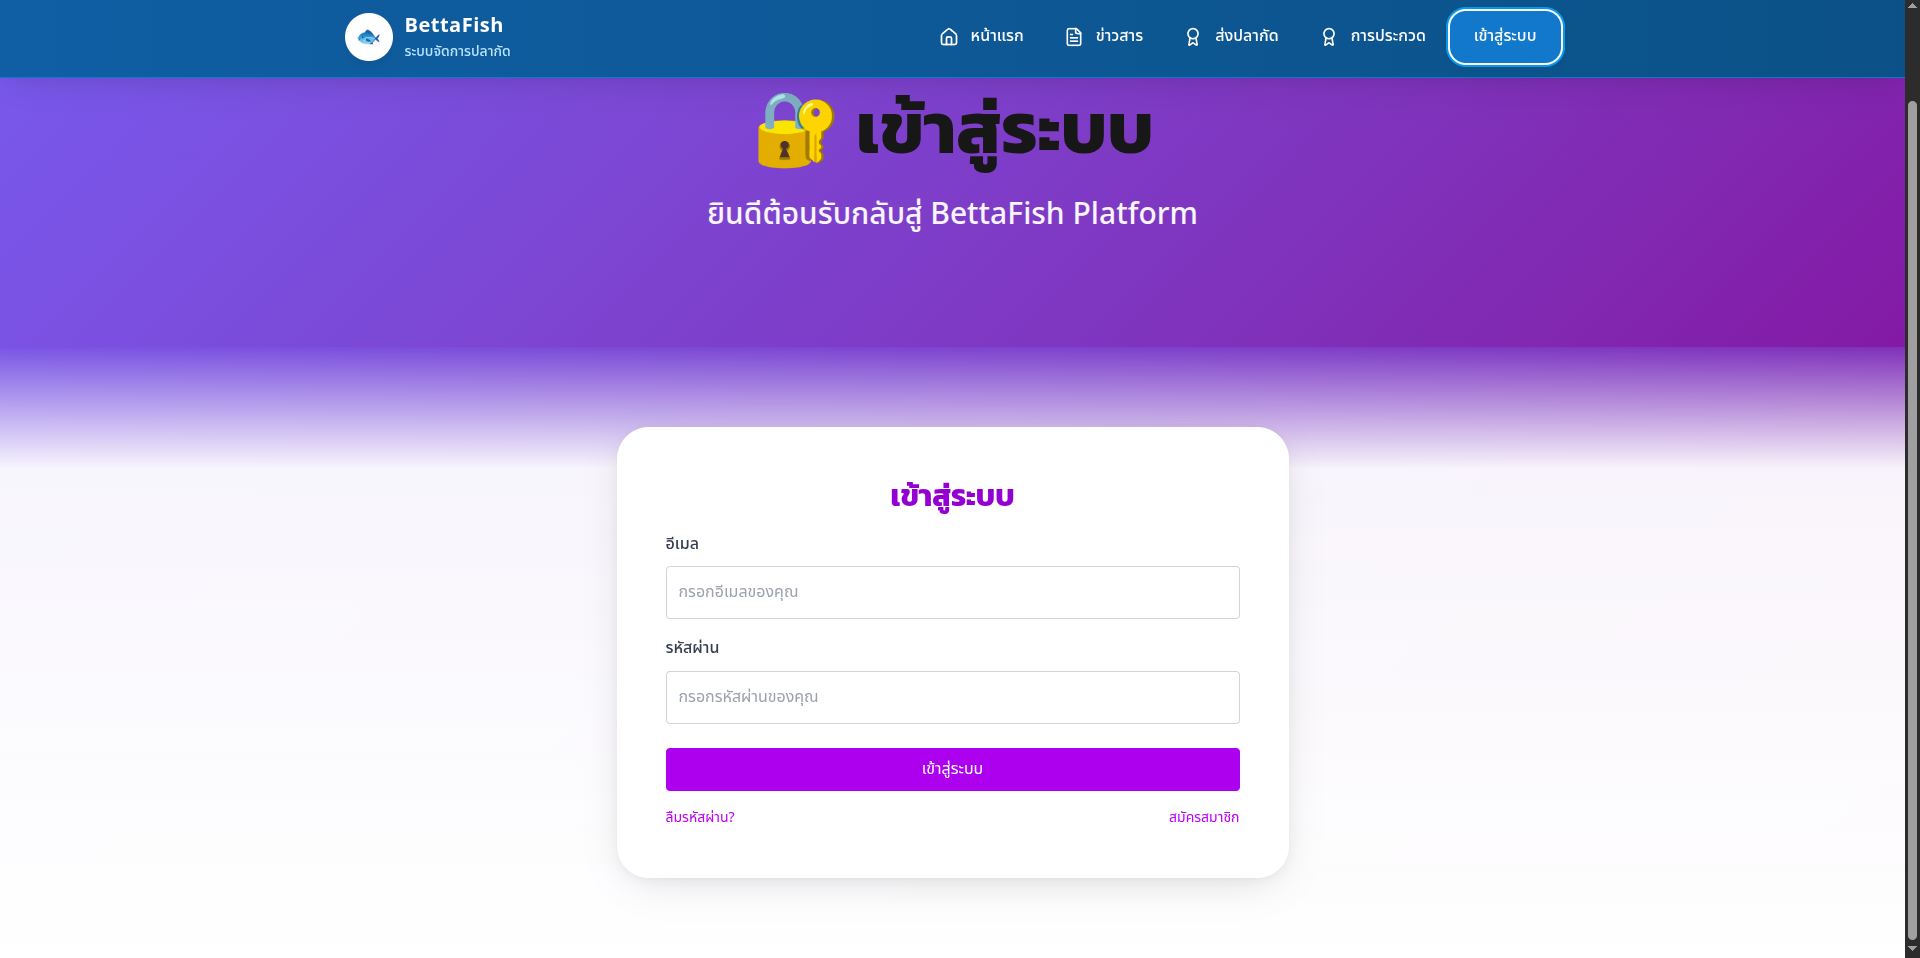
\includegraphics[width=0.8\linewidth]{LG1}
	\caption{หน้าเข้าสู่ระบบ}
\end{figure}

\noindent{\bfseries\fontsize{16pt}{19.2pt}\selectfont วิธีใช้งานหน้าเข้าสู่ระบบ}\par

\begin{sloppypar}
	\begin{enumerate}
		\item เตรียม อีเมลหรือชื่อผู้ใช้ และ รหัสผ่าน ที่ลงทะเบียนไว้
		\item หากยังไม่มีบัญชี ให้กด “สมัครสมาชิก” ด้านล่างฟอร์ม
	\end{enumerate}
\end{sloppypar}

\noindent{\bfseries\fontsize{16pt}{19.2pt}\selectfont ขั้นตอนใช้งาน}\par

\begin{sloppypar}
	\begin{enumerate}
		\item เปิดหน้า เข้าสู่ระบบ (Login)
		\item ที่ช่อง อีเมลหรือชื่อผู้ใช้ พิมพ์อีเมลหรือชื่อผู้ใช้ของคุณ
		\item ที่ช่อง รหัสผ่าน พิมพ์รหัสผ่านของคุณ
		\item กดปุ่ม “เข้าสู่ระบบ” หรือกดปุ่ม Enter
	\end{enumerate}
\end{sloppypar}

\newpage

\vspace{\baselineskip}

\begin{figure}[h]
	\centering
	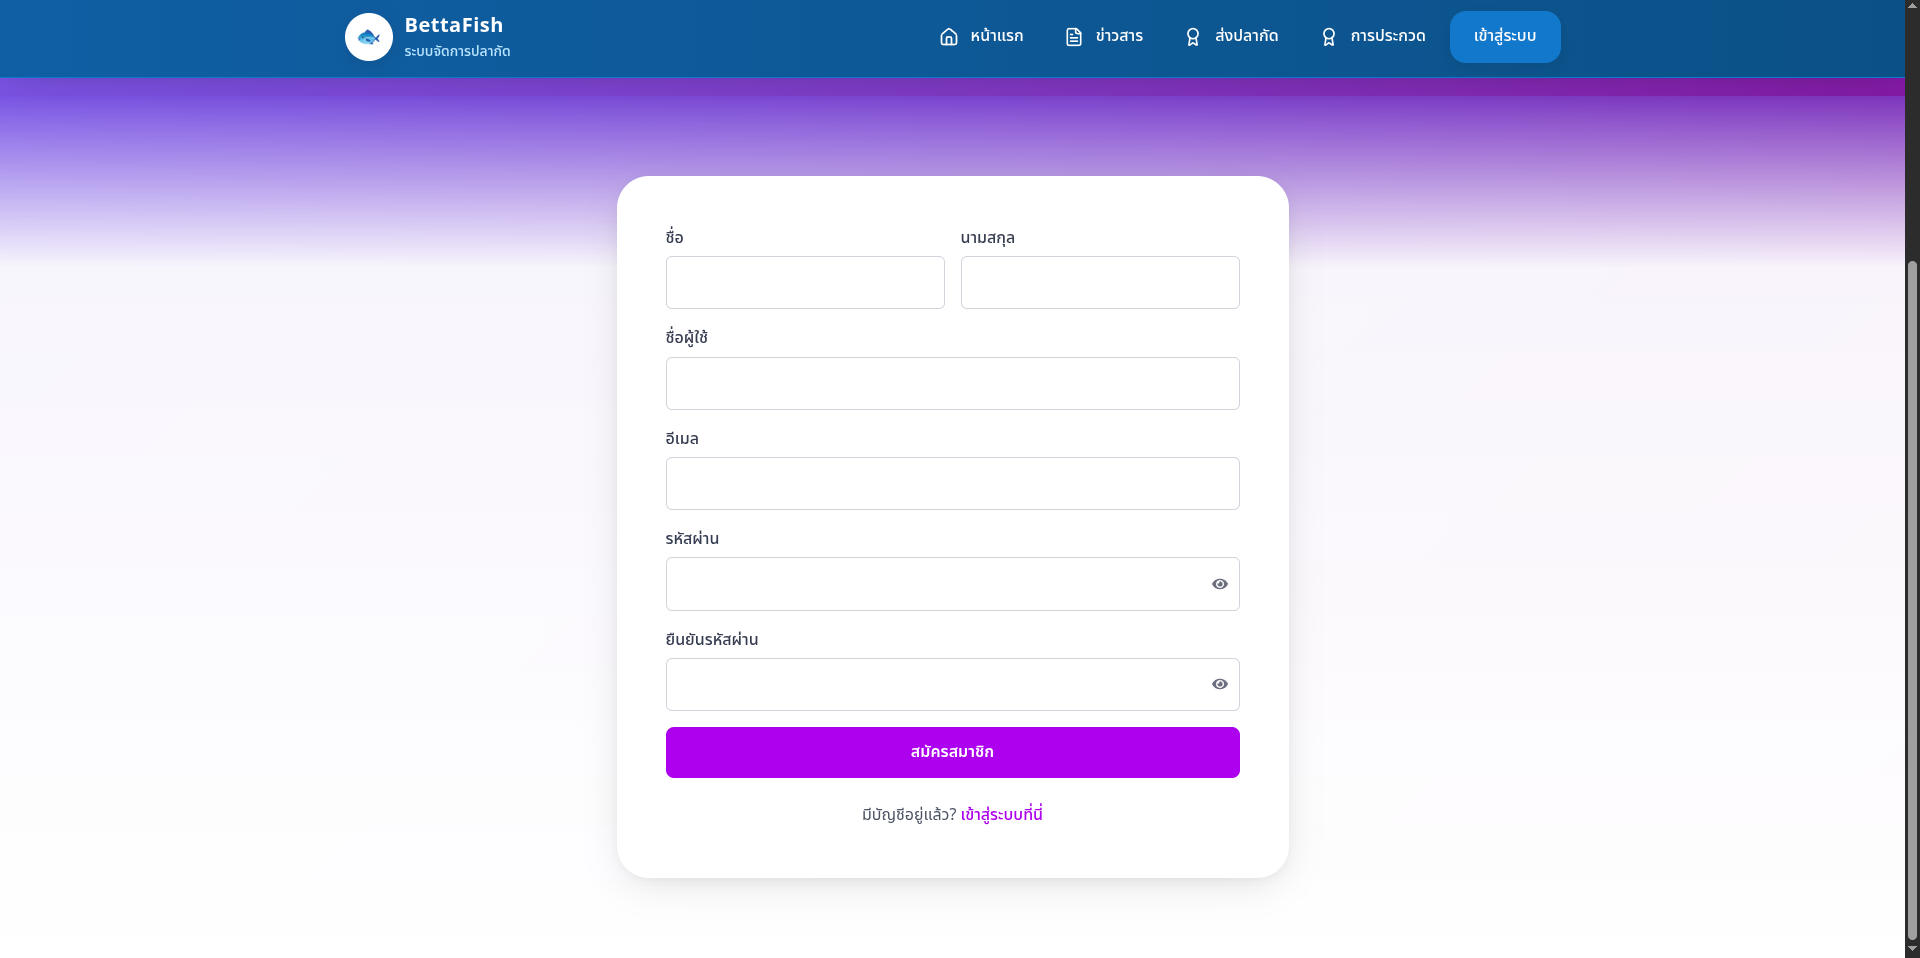
\includegraphics[width=0.8\linewidth]{RG1}
	\caption{หน้าสมัครสมาชิก}
\end{figure}

\noindent{\bfseries\fontsize{16pt}{19.2pt}\selectfont วิธีใช้งานหน้าหน้าสมัครสมาชิก}\par

\begin{sloppypar}
	\begin{enumerate}
		\item ใช้สำหรับสร้างบัญชีใหม่บนแพลตฟอร์ม
		\item กรอกข้อมูลตามช่องต่อไปนี้ให้ครบถ้วน
		\begin{enumerate}
			\item ชื่อ และ นามสกุล
			\item ชื่อผู้ใช้ (อย่างน้อย 3 ตัวอักษร)
			\item อีเมล (รูปแบบอีเมลที่ถูกต้อง)
			\item รหัสผ่าน (อย่างน้อย 6 ตัวอักษร)
			\item ยืนยันรหัสผ่าน (ต้องตรงกับรหัสผ่าน)
		\end{enumerate}
		\item ไอคอนรูปตาในช่องรหัสผ่านใช้เพื่อ แสดง/ซ่อน รหัสผ่านได้
		\item เมื่อกดส่งฟอร์ม ระบบจะป้องกันการกดซ้ำและแสดงสถานะ “กำลังดำเนินการ...”
		\item หากสมัครสำเร็จ จะมีแจ้งเตือนและพาไปหน้า เข้าสู่ระบบ 
		\item หากมีบัญชีอยู่แล้ว กดลิงก์ “เข้าสู่ระบบที่นี่” ด้านล่างฟอร์ม
	\end{enumerate}
\end{sloppypar}

\noindent{\bfseries\fontsize{16pt}{19.2pt}\selectfont ขั้นตอนใช้งาน}\par


\begin{sloppypar}
	\begin{enumerate}
		\item เปิดหน้า สมัครสมาชิก
		\item กรอก ชื่อ และ นามสกุล
		\item กรอก ชื่อผู้ใช้ (≥ 3 ตัวอักษร)
		\item กรอก อีเมล ให้ถูกต้องตามรูปแบบ
		\item กรอก รหัสผ่าน (≥ 6 ตัวอักษร)
		\begin{enumerate}
			\item หากต้องการตรวจสอบตัวสะกด กดไอคอนรูปตาเพื่อแสดงรหัสผ่าน
		\end{enumerate}
		\item กรอก ยืนยันรหัสผ่าน ให้ ตรงกับรหัสผ่าน
		\item กดปุ่ม “สมัครสมาชิก”
		\begin{enumerate}
			\item ถ้าข้อมูลไม่ครบ/ไม่ถูกต้อง ระบบจะแสดงข้อความสีแดงใต้ช่องนั้น ๆ ให้แก้ไขแล้วกดส่งใหม่
		\end{enumerate}
		\item เมื่อสมัครสำเร็จ รอแจ้งเตือน แล้วระบบจะพาไปหน้า เข้าสู่ระบบ โดยอัตโนมัติ
	\end{enumerate}
\end{sloppypar}

\begin{figure}[h]
	\centering
	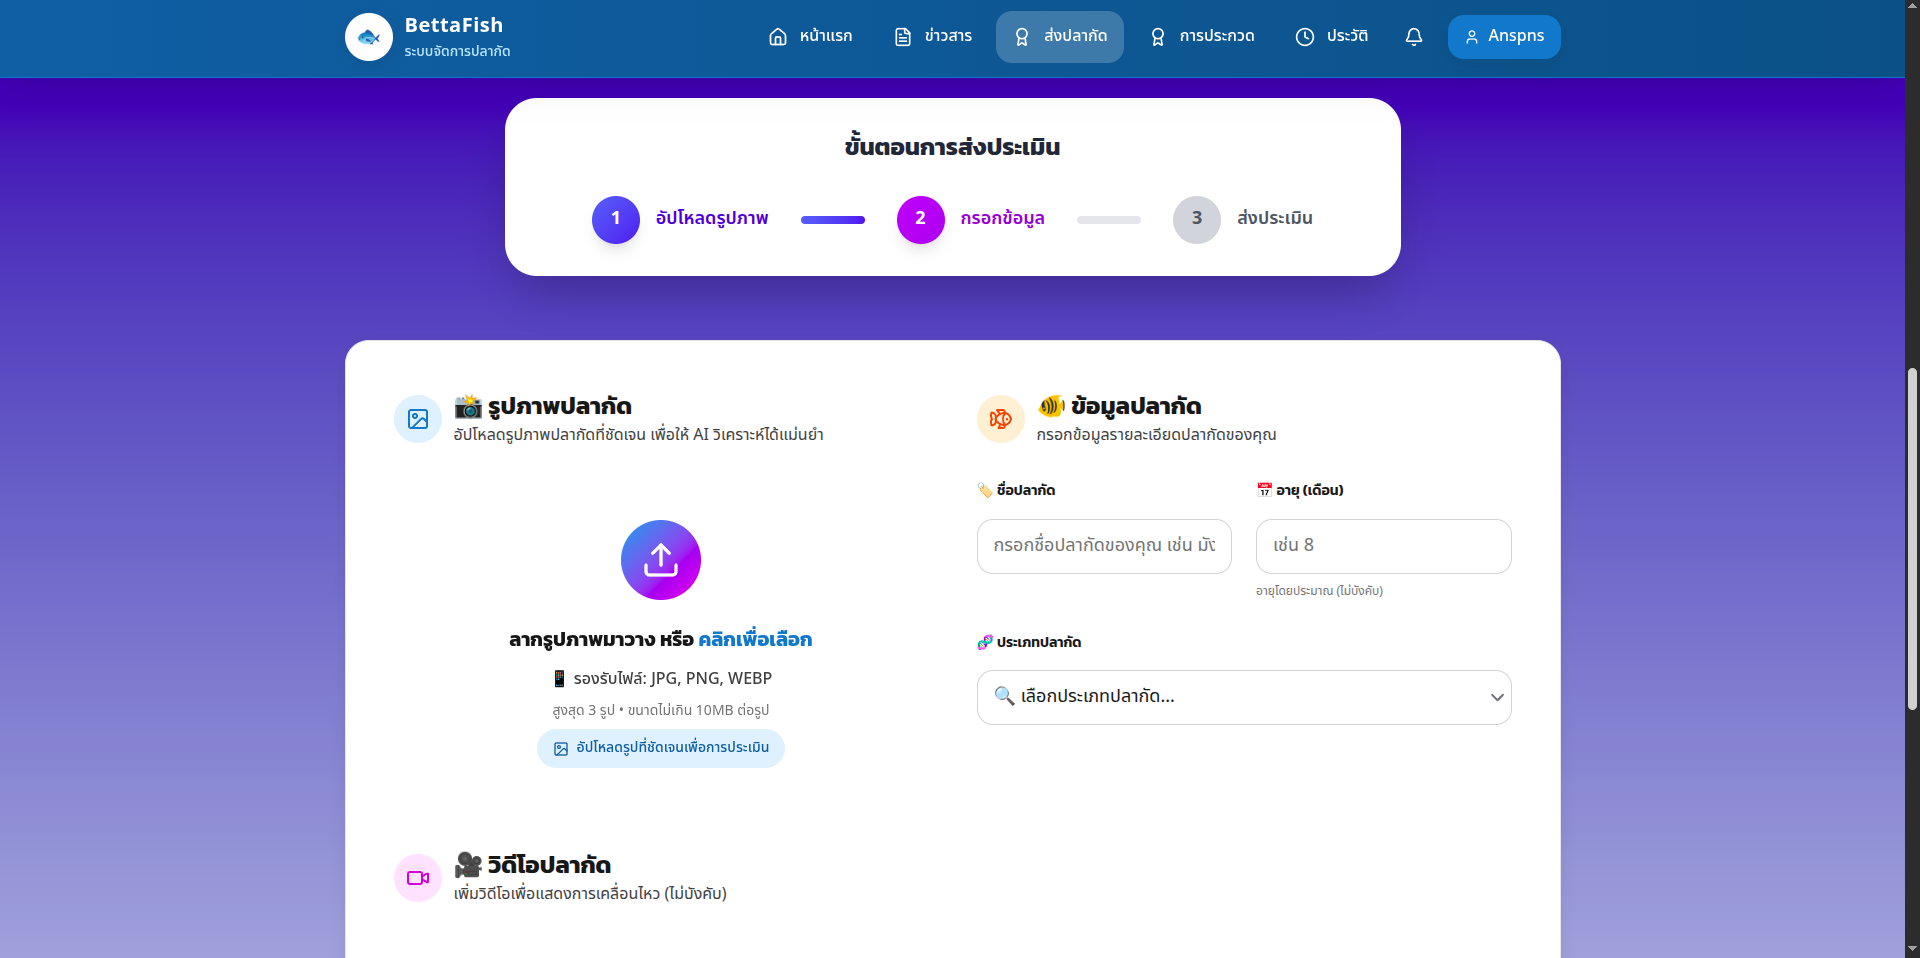
\includegraphics[width=0.8\linewidth]{EV1}
	\caption{หน้าส่งปลากัดเพื่อประเมินคุณภาพ}
\end{figure}

\noindent{\bfseries\fontsize{16pt}{19.2pt}\selectfont วิธีใช้งานหน้าส่งปลากัดเพื่อประเมินคุณภาพ}\par

\begin{sloppypar}
	\begin{enumerate}
		\item ต้องอัปโหลด รูปปลากัดให้ครบ 3 รูป (JPG/PNG/WEBP) — ระบบ AI จะตรวจสอบว่าทั้ง 3 รูปเป็น ประเภทเดียวกัน
		\begin{enumerate}
			\item ถ้าพบรูปที่วิเคราะห์ไม่ได้/คนละประเภท ระบบจะ ลบเฉพาะรูปนั้น และแจ้งเตือนให้อัปโหลดใหม่
		\end{enumerate}
		\item วิดีโอเป็น ตัวเลือกเสริม (MP4/MOV/AVI) เพื่อแสดงการเคลื่อนไหว (แนะนำ ≤ 50MB)
		\item กรอกข้อมูลปลา: ชื่อปลากัด, อายุ (เดือน – ไม่บังคับ), ประเภทปลากัด
		\begin{enumerate}
			\item AI จะเสนอประเภทให้อัตโนมัติเมื่อรูปครบ 3 รูป; หากเลือกต่างจากที่ AI แนะนำ ระบบจะถามยืนยันอีกครั้ง
		\end{enumerate}
		\item ปุ่ม “ส่ง” จะกดได้เมื่อ อัปโหลดรูปครบ 3 รูป และ AI ตรวจสอบเสร็จ แล้วเท่านั้น
		\item ก่อนส่งจริง จะมี หน้าต่างยืนยัน แสดงสรุปข้อมูล (เช่น ประเภท/ชื่อปลา) ให้ตรวจทาน
	\end{enumerate}
\end{sloppypar}

\noindent{\bfseries\fontsize{16pt}{19.2pt}\selectfont ขั้นตอนใช้งาน}\par


\begin{sloppypar}
	\begin{enumerate}
		\item ที่ส่วน รูปภาพปลากัด ให้ ลาก-วาง หรือ กดคลิกเพื่อเลือกไฟล์ จน ครบ 3 รูป
		\begin{enumerate}
			\item ตรวจสอบตัวอย่างรูปที่อัปโหลดด้านล่าง และลบรูปใด ๆ ด้วยปุ่ม x หากต้องการเปลี่ยน
		\end{enumerate}
		\item รอระบบ AI ตรวจสอบ ความตรงกันของ 3 รูป (จะมีสถานะกำลังตรวจสอบ และแสดงเปอร์เซ็นต์ความมั่นใจเมื่อเสร็จ)
		\item (ไม่บังคับ) อัปโหลด วิดีโอปลากัด เพื่อเสริมการประเมิน แล้วกดเล่นเช็คตัวอย่างได้
		\item ที่ส่วน ข้อมูลปลากัด
		\item ตรวจสอบแถบแจ้งเตือนด้านล่างปุ่มส่ง
		\begin{enumerate}
			\item กรอก ชื่อปลากัด
			\item กรอก อายุ (เดือน) หากทราบ
			\item เลือก ประเภทปลากัด (ระบบมักเติมตามที่ AI แนะนำให้แล้ว)
			\item หากเลือกต่างจาก AI ระบบจะแสดง หน้าต่างยืนยันการเปลี่ยนประเภท
		\end{enumerate}
		\item กดปุ่ม “ส่งประเมินปลากัด” หรือ “ส่งเข้าร่วมประกวด” (ตามโหมด)
		\begin{enumerate}
			\item ถ้ายังไม่ครบ 3 รูป  ระบบจะแจ้งให้ อัปโหลดเพิ่ม
			\item ถ้า AI ยังไม่เสร็จ  ระบบจะแจ้งให้ รอการตรวจสอบ
		\end{enumerate}
		\item ในหน้าต่างยืนยัน ให้ตรวจทานข้อมูล แล้วกด “ยืนยันการส่ง”
		\begin{enumerate}
			\item ระบบจะแสดงสถานะ กำลังส่ง… และเมื่อสำเร็จจะแจ้งเตือน พร้อมพาไปหน้า ประวัติการส่ง
		\end{enumerate}
	\end{enumerate}
\end{sloppypar}

\newpage

\begin{figure}[h]
	\centering
	\includegraphics[width=0.8\linewidth]{HP5}
	\caption{หน้ารวมการประกวดปลากัด}
\end{figure}

\noindent{\bfseries\fontsize{16pt}{19.2pt}\selectfont วิธีใช้งานหน้าหน้ารวมการประกวดปลากัด}\par

\begin{sloppypar}
	\begin{enumerate}
		\item หน้านี้แสดง รายการการประกวดทั้งหมด เป็นการ์ด พร้อมโปสเตอร์ (ถ้าไม่มีจะแสดงภาพแทน), ชื่อ, คำอธิบายย่อ, และช่วงวันที่จัดงาน
		\item ที่มุมซ้ายบนรูป จะมี ป้ายสถานะ อัปเดตอัตโนมัติ
		\begin{enumerate}
			\item กำลังจะเริ่ม = ยังไม่ถึงวันเริ่ม
			\item เปิดรับสมัคร = อยู่ในช่วงเริ่ม–สิ้นสุด
			\item สิ้นสุดแล้ว = เลยวันสิ้นสุด
			\item กำลังดำเนินการ = ไม่เข้ากรณีข้างต้น
		\end{enumerate}
		\item คลิกที่การ์ดเพื่อไปหน้า รายละเอียดการประกวด
		\item หากกดสมัครจากปุ่ม/ลิงก์ที่เกี่ยวข้องและคุณ เข้าสู่ระบบแล้ว จะเปิด หน้าต่างสมัคร (Modal) ถ้ายัง ไม่ได้ล็อกอิน ระบบจะพาไปหน้า เข้าสู่ระบบ ก่อน
	\end{enumerate}
\end{sloppypar}

\noindent{\bfseries\fontsize{16pt}{19.2pt}\selectfont ขั้นตอนใช้งาน}\par

\begin{sloppypar}
	\begin{enumerate}
		\item เปิดหน้า การประกวดปลากัด
		\item เลื่อนดูรายการการประกวด และสังเกต ป้ายสถานะ บนรูปโปสเตอร์
		\item คลิกการ์ดที่สนใจเพื่อดู รายละเอียดเพิ่มเติม
		\item หากต้องการสมัคร
		\begin{enumerate}
			\item ถ้า ล็อกอินแล้ว: ระบบเปิด หน้าต่างสมัคร ให้กรอกข้อมูลและอัปโหลดสื่อ
			\item ถ้า ยังไม่ล็อกอิน: ระบบจะพาไปหน้า เข้าสู่ระบบ แล้วกลับมาทำรายการต่อ
		\end{enumerate}
		\item กลับมาที่หน้านี้เมื่อไหร่ก็ได้ เพื่อดูรายการใหม่ ๆ หรือสถานะที่อัปเดตแล้ว
	\end{enumerate}
\end{sloppypar}

\newpage

\begin{figure}[h]
	\centering
	\includegraphics[width=0.8\linewidth]{HP6}
	\caption{หน้าต่างสมัครเข้าร่วมประกวด}
\end{figure}


\noindent{\bfseries\fontsize{16pt}{19.2pt}\selectfont วิธีใช้งานหน้าต่างสมัครเข้าร่วมประกวด}\par

\begin{sloppypar}
	\begin{enumerate}
		\item ใช้สำหรับ ส่งปลากัดเข้าร่วมการประกวด ภายในหน้าต่าง (Modal) เดียว
		\item กรอกข้อมูลหลัก: ชื่อปลากัด, อายุ (เดือน–ไม่บังคับ), ประเภทปลากัด
		\begin{enumerate}
			\item ถ้าเวทีนี้กำหนดประเภทเดียว ปุ่มเลือกประเภทจะ ล็อกอัตโนมัติ
		\end{enumerate}
		\item อัปโหลดสื่อ
		\begin{enumerate}
			\item รูปภาพ ได้สูงสุด 3 รูป (JPG/PNG/WebP) พร้อมแสดงตัวอย่างและปุ่มลบ
			\item วิดีโอ (ไม่บังคับ) รองรับ MP4/WebM/QuickTime พร้อมตัวอย่างและปุ่มลบ
		\end{enumerate}
		\item ระบบมี AI ตรวจเช็กแบบสด จากรูปและประเภทที่เลือก
		\begin{enumerate}
			\item จะแจ้งว่า ตรงเงื่อนไข หรือ ไม่ตรงเงื่อนไขแต่ยังส่งได้ หรือ ไม่มั่นใจ
		\end{enumerate}
		\item ต้องติ๊ก ยืนยันความถูกต้องของข้อมูล ก่อนกด “ยืนยันการสมัคร”
		\item กดปุ่ม X มุมขวาบนเพื่อปิดหน้าต่างโดยไม่ส่งข้อมูล
	\end{enumerate}
\end{sloppypar}

\noindent{\bfseries\fontsize{16pt}{19.2pt}\selectfont ขั้นตอนใช้งาน}\par


\begin{sloppypar}
	\begin{enumerate}
		\item เปิดหน้าต่าง สมัครเข้าร่วมประกวด
		\item กรอก ชื่อปลากัด และ (ถ้ามี) อายุ (เดือน)
		\item เลือก ประเภทปลากัด (ถ้าถูกล็อกแสดงว่าเวทีกำหนดประเภทเดียว)
		\item อัปโหลด รูปภาพ โดยลาก–วาง หรือคลิกเลือก (แนะนำอัปอย่างน้อย 1 รูป และได้สูงสุด 3 รูป)
		\begin{enumerate}
			\item ตรวจดูตัวอย่างรูป และกดปุ่ม ลบ (x) หากต้องการเปลี่ยน
		\end{enumerate}
		\item (ไม่บังคับ) อัปโหลด วิดีโอ เพื่ือแสดงการเคลื่อนไหว
		\item รอสถานะ AI กำลังตรวจสอบ… แล้วดูผลลัพธ์ว่า ตรงเงื่อนไข / ไม่ตรง / ไม่มั่นใจ
		\item ติ๊กช่อง ยืนยันการส่งข้อมูลเข้าร่วมประกวด
		\item กดปุ่ม ยืนยันการสมัคร
		\begin{enumerate}
			\item ขณะส่ง ระบบจะแสดง กำลังส่งข้อมูล… และแจ้งผลสำเร็จ/ข้อผิดพลาดด้วยการแจ้งเตือน (toast)
		\end{enumerate}
	\end{enumerate}
\end{sloppypar}


\begin{figure}[h]
	\centering
	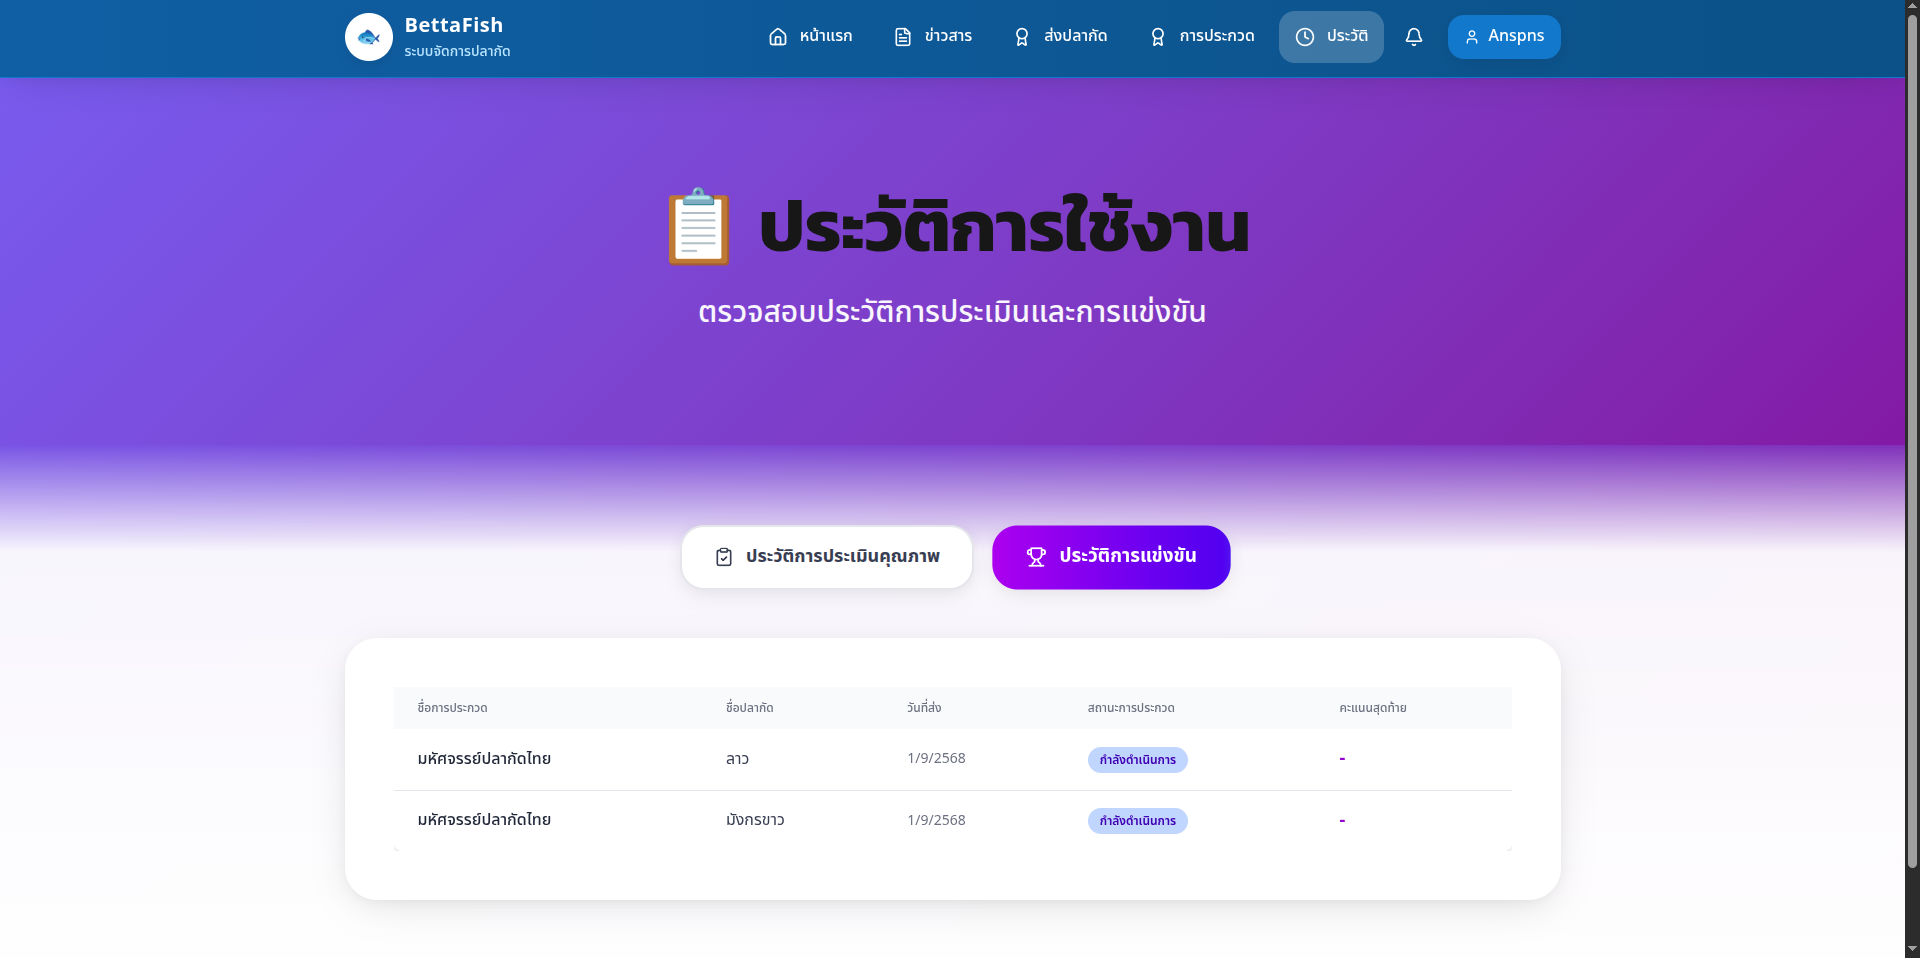
\includegraphics[width=0.8\linewidth]{HT2}
	\caption{หน้าประวัติการเข้าร่วมการแข่งขัน}
\end{figure}

\noindent{\bfseries\fontsize{16pt}{19.2pt}\selectfont วิธีใช้งานหน้าประวัติการเข้าร่วมการแข่งขัน}\par

\begin{sloppypar}
	\begin{enumerate}
		\item หน้านี้จะแสดง ประวัติที่คุณส่งปลากัดเข้าร่วมการแข่งขัน ในรูปแบบตาราง
		\item รายการแต่ละแถวมีข้อมูล: ชื่อการประกวด, ชื่อปลากัด, วันที่ส่ง, สถานะการแข่งขัน, สถานะการสมัคร, คะแนน, ปุ่มดูรายละเอียด
		\item ป้ายสถานะ (Badge) จะแสดงด้วยสีอ่านง่าย
		\begin{enumerate}
			\item สถานะการแข่งขัน: กำลังดำเนินการ, ปิดรับสมัคร, ตัดสิน, ประกาศผล, ยกเลิก ฯลฯ
			\item สถานะการสมัคร: รอตรวจสอบ, ผ่านการคัดเลือก, ประกาศผล, ถูกปฏิเสธ
		\end{enumerate}
		\item กด ดูรายละเอียด เพื่อเปิดหน้าต่าง (Modal) แสดงข้อมูลเชิงลึก เช่น ภาพ/วิดีโอ คะแนน เหตุผลการปฏิเสธ ฯลฯ
		\item ถ้าไม่มีรายการ ระบบจะแจ้งว่า ยังไม่มีประวัติ
		\item ขณะโหลดข้อมูลจะขึ้นข้อความ กำลังโหลด… และถ้าเกิดปัญหาจะแสดง ข้อความผิดพลาด
	\end{enumerate}
\end{sloppypar}

\noindent{\bfseries\fontsize{16pt}{19.2pt}\selectfont ขั้นตอนใช้งาน}\par

\begin{sloppypar}
	\begin{enumerate}
		\item เปิดหน้า ประวัติการเข้าร่วมการแข่งขัน
		\item รอให้ระบบ โหลดข้อมูล (หากช้าเล็กน้อยเป็นปกติ)
		\item ดูภาพรวมจากตาราง
		\begin{enumerate}
			\item เช็ค ชื่อการประกวด / ชื่อปลากัด / วันที่ส่ง
			\item ดู สถานะการแข่งขัน และ สถานะการสมัคร จากป้ายสี
			\item ตรวจสอบ คะแนน (ถ้ามี)
		\end{enumerate}
		\item ต้องการดูรายละเอียดเพิ่มเติม ให้กดปุ่ม ดูรายละเอียด ที่แถวรายการนั้น
		\item ภายในหน้าต่างรายละเอียด ตรวจสอบข้อมูลรูป/วิดีโอ คะแนน และเหตุผลต่าง ๆ จากนั้นกดปิดเพื่อกลับสู่ตาราง
		\item หากตารางว่าง ให้กลับไปหน้า การประกวด เพื่อสมัครรายการใหม่ เมื่อมีผลส่งแล้วจะมาแสดงที่หน้านี้อัตโนมัติ
	\end{enumerate}
\end{sloppypar}

\begin{figure}[h]
	\centering
	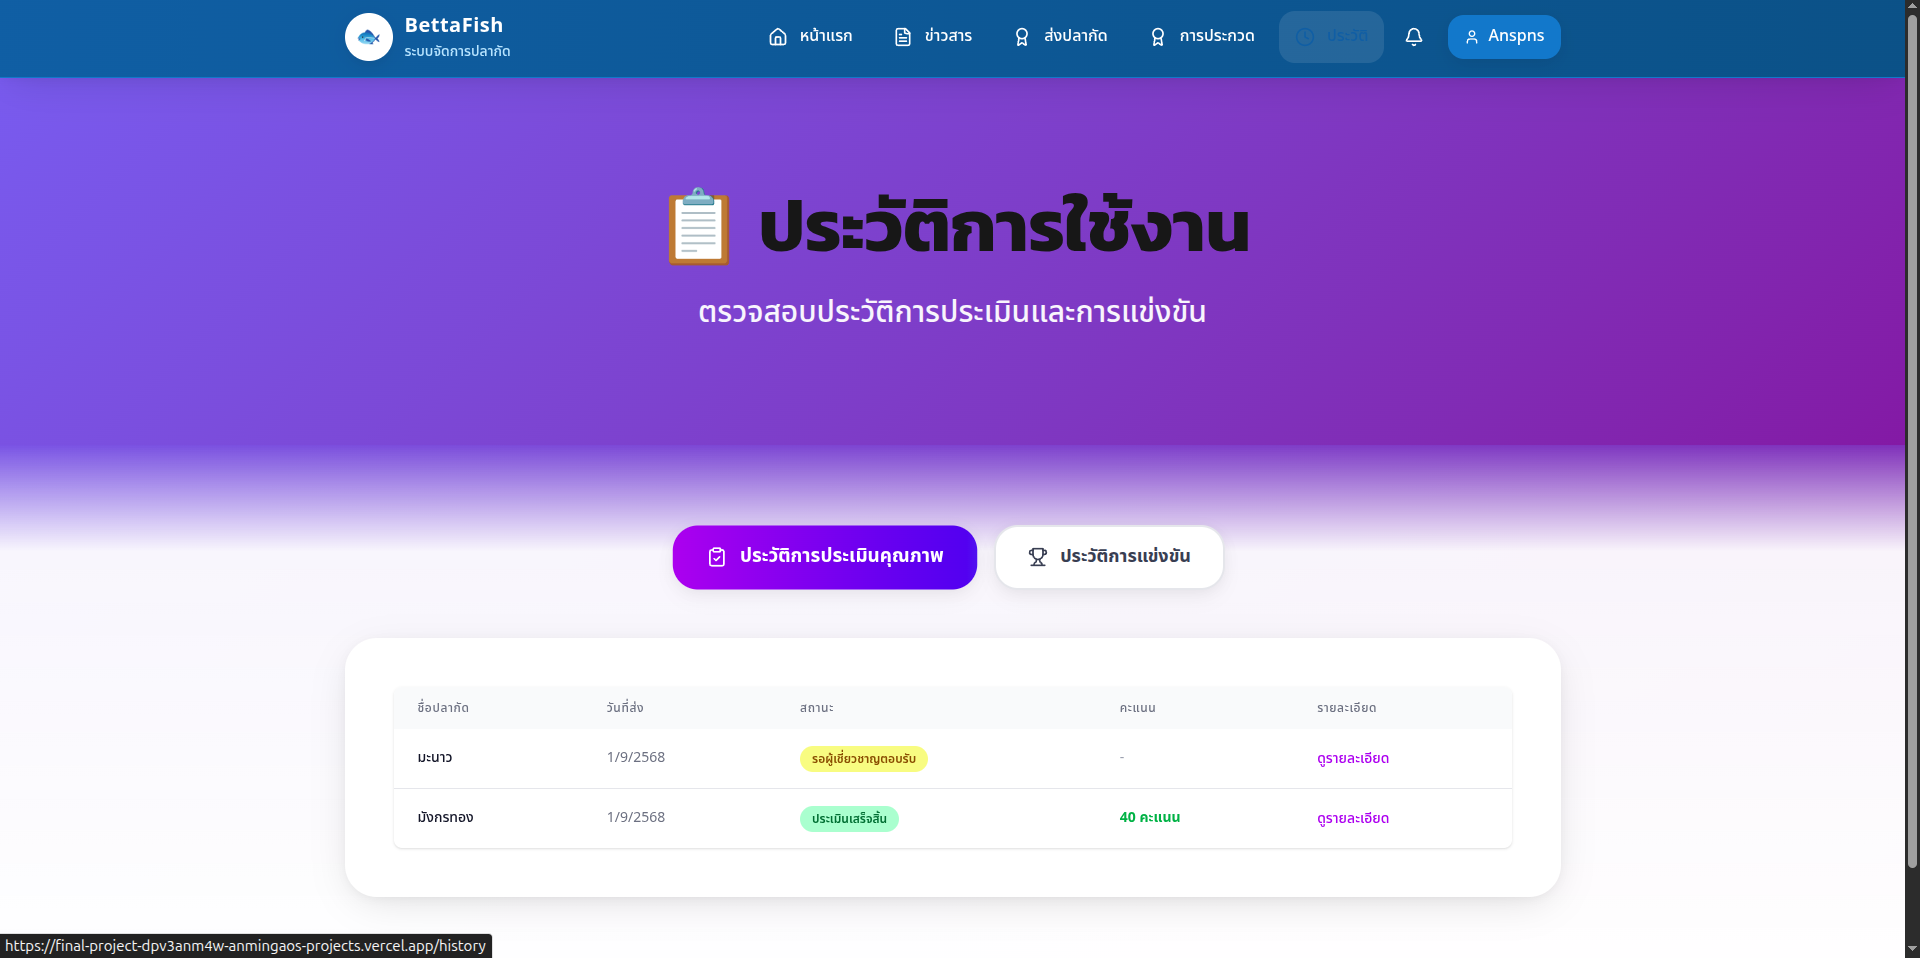
\includegraphics[width=0.8\linewidth]{HT1}
	\caption{หน้าประวัติการประเมินคุณภาพ}
\end{figure}

\noindent{\bfseries\fontsize{16pt}{19.2pt}\selectfont วิธีใช้งานหน้าประวัติการประเมินคุณภาพ}\par

\begin{sloppypar}
	\begin{enumerate}
		\item หน้านี้แสดง ประวัติการส่งประเมินคุณภาพปลากัด ของคุณในรูปแบบตาราง
		\item ระหว่างโหลดข้อมูลจะแสดง สัญลักษณ์หมุน (Loader) และหากเกิดปัญหาจะแสดง กล่องข้อความผิดพลาด
		\item เมื่อไม่มีข้อมูล จะแสดงข้อความ “ยังไม่มีประวัติการประเมินคุณภาพ”
		\item คอลัมน์ในตาราง
		\begin{enumerate}
			\item ชื่อปลากัด
			\item วันที่ส่ง (รูปแบบวันที่ไทย)
			\item สถานะ (แสดงเป็นป้ายสี เช่น รอการตรวจสอบ/กำลังประเมิน/ประเมินเสร็จสิ้น/ถูกปฏิเสธ ฯลฯ)
			\item คะแนน (ถ้ามีจะแสดงเป็นตัวหนาสีเขียว มิฉะนั้นเป็น “-”)
			\item รายละเอียด (ปุ่มเปิดดูข้อมูลเชิงลึก)
		\end{enumerate}
		\item ปุ่ม ดูรายละเอียด จะเปิดหน้าต่าง (Modal) แสดงข้อมูลฉบับเต็มของการประเมิน
	\end{enumerate}
\end{sloppypar}

\noindent{\bfseries\fontsize{16pt}{19.2pt}\selectfont ขั้นตอนใช้งาน}\par

\begin{sloppypar}
	\begin{enumerate}
		\item เข้าหน้า ประวัติการประเมินคุณภาพ
		\item รอให้ระบบ โหลดข้อมูล (หากมีปัญหาจะเห็นข้อความแจ้งข้อผิดพลาด)
		\item ตรวจดูตาราง
		\begin{enumerate}
			\item เช็ค ชื่อปลากัด และ วันที่ส่ง
			\item ดู สถานะ จากป้ายสี และ คะแนน หากมี
		\end{enumerate}
		\item กด ดูรายละเอียด ในแถวที่ต้องการ เพื่อเปิด หน้าต่างรายละเอียด
		\item อ่านข้อมูลเชิงลึกใน Modal แล้ว ปิดหน้าต่าง เพื่อกลับสู่ตาราง
		\item หากยังไม่มีรายการ ให้กลับไปหน้า ส่งประเมินคุณภาพ ก่อน แล้วข้อมูลจะมาแสดงในหน้านี้โดยอัตโนมัติ
	\end{enumerate}
\end{sloppypar}

\clearpage